\documentclass[a4paper,12pt]{article} 
\usepackage[T2A]{fontenc}			
\usepackage[utf8]{inputenc}			
\usepackage[english,russian]{babel}	
\usepackage{amsmath,amsfonts,amssymb,amsthm,mathrsfs,mathtools} 
\usepackage{cancel}
\usepackage{hhline}
\usepackage{multirow}
\usepackage[colorlinks, linkcolor = purple, citecolor = purple]{hyperref}
\usepackage{upgreek}\usepackage[left=2cm,right=2cm,top=2cm,bottom=3cm,bindingoffset=0cm]{geometry}
\usepackage{tikz}
\usepackage{graphicx}
\usepackage{subfig}
\usepackage{titletoc}
\usepackage{pgfplots}
\usepackage{xcolor}
\usepackage{wrapfig}

\newcommand{\angstrom}{\text{\normalfont\AA}}
\author{Тимофей Черников\\
Группа Б05-902}
\title{5.10.1 Электронный парамагнитный резонанс.}
\date{}

\begin{document}
\maketitle
\textbf{В работе}: исследуется электронный парамагнитный резонанс (ЭПР) в молекуле дифенилпикрилгидразила (ДФПГ), 
определяется $g$-фактор электрона, измеряется ширина линий ЭПР.


\section*{Теория}
    С помощью метода ЭПР изучается резонансное поглощение электромагнитного поля поля в образце в зависимости от условий,
    задаваемых экспериментатором: постоянного магнитного поля, частоты колебаний переменного поля, температуры и других.
    Простейшей моделью для рассмотрения ЭПР является система из невзаимодействующих
    частиц со спином $S = 1/2$, помещённая во внешнее магнитное поле. В отсутствие
    магнитного поля энергии состояний с проекцией спина $S_Z = \pm 1/2$ совпадают. 
    Из-за эффекта Зеемана происходит расщепление линий атомных спектров и энергии состояний с различными проекциями спина начинают различаться. 
    Если направить на нашу систему поток излучения с энергией, равной разнице энергий этих состояний 

    \begin{equation}\label{2}
    h \nu = g\mu_B B,
    \end{equation} 

    то станут возможны индуцированные переходы между состояниями. 
    Эти переходы происходят с поглощением или испусканием фотона в зависимости от того, 
    в каком из состояний была система до взаимодействия с излучением. 
    В состоянии теплового равновесия нижний энергетический уровень более заселён, 
    поэтому наблюдается поглощение электромагнитного излучения. \\
    \section*{Описание установки}
    \begin{wrapfigure}{r}{0.5\textwidth}
        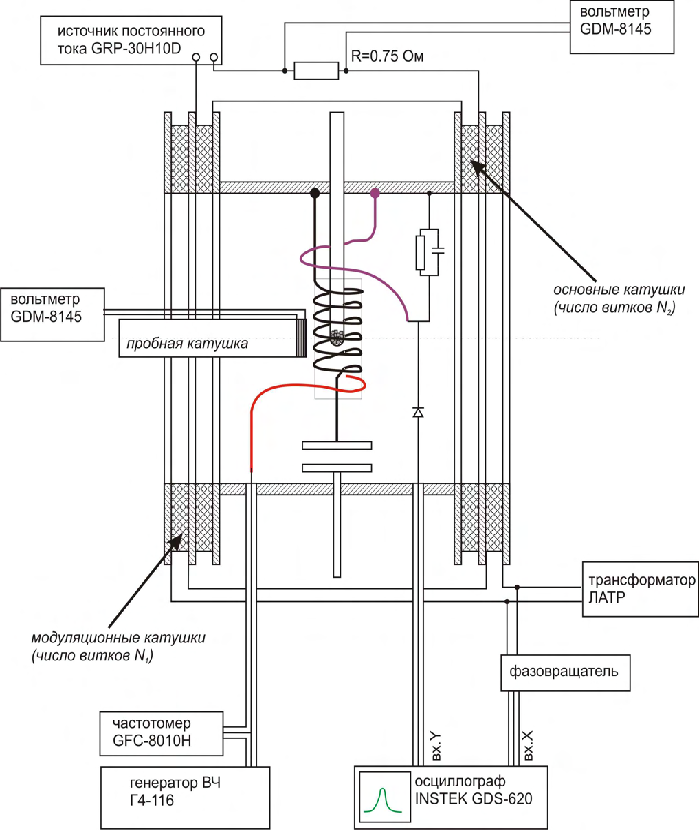
\includegraphics[width = 0.5\textwidth]{ustanovka.pdf}
        \centering
    \caption{Схема установки.}
    \end{wrapfigure}
    Схема установки представлена на Рис. 1. Образец (порошок ДФПГ) в стеклянной ампуле помещается внутрь катушки индуктивности, входящей в состав колебательного контура. Входящий в состав контура конденсатор состоит из двух пластин, разделённых воздушным зазором, одна из пластин может перемещаться поворотом штока. Колебания в контуре возбуждаются антенной, соединённой с генератором высокой частоты (ВЧ) Г4-116. Амплитуда колебаний поля в катушке индуктивности
    измеряется по наводимой в петле связи ЭДС индукции. Высокочастотные колебания ЭДС
    индукции в приёмном контуре детектируются диодом, измеряемая при помощи
    осциллографа низкочастотная огибающая этого сигнала пропорциональна квадрату
    амплитуды колебаний поля в катушке.\\
    Постоянное магнитное поле создаётся пропусканием тока от источника постоянного тока через основные катушки. При этом при помощи вольтметра измеряется падение напряжения на резисторе в цепи основных катушек. Переменное поле небольшой амплитуды создаётся подачей на модуляционные катушки напряжения с регулируемого трансформатора ЛАТР. Для измерения амплитуды колебаний переменного поля используется пробная катушка известной геометрии, подключённая к вольтметру. Пусть поток через неё $\Phi_{\text{проб}}$, тогда ЭДС индукции
    \[\mathcal{E} = - \dfrac{d\Phi_{\text{проб}}}{dt}.\]
    Если $I_{\text{осн}}$ -- ток через основную катушку, а $M$ -- взаимная индуктивность основной и пробной катушек, то
    \[\Phi_{\text{проб}} = M I_{\text{осн}}.\]
    Тогда амплитудное значение ЭДС индукции
    \[\mathcal{E}_{\text{амп}} = - \dfrac{dM I_{\text{осн}}}{dt} = M \omega I_{\text{амп}}.\]
    Учитывая, что $I_{\text{амп}} = \sqrt{2} I_{\text{действ}}=\frac{V_r}{r}$, где $V_R$, $R$ -- напряжение на резисторе с сопротивлением $R$ в цепи основных катушек, а также $\mathcal{E}_{\text{амп}} = \sqrt{2}\mathcal{E}_{\text{ср}}$, получим
    \[\mathcal{E}_{\text{ср}} = M \omega \dfrac{V_R}{R} = k V_R.\]
    Тогда, зная, что
    \[\Phi_{\text{проб}} = B_0 N_{\text{проб}} \dfrac{\pi d_{\text{проб}}^2}{4} =  \dfrac{MU_R}{R} = \dfrac{k U}{\omega},\]
    где $U$ -- напряжение на $R$ в резонансе, получим
    \begin{equation}\label{1}
    B_0 = \dfrac{4k U}{\pi \omega d^2_{\text{проб}} N_{\text{проб}}}.
    \end{equation}
    Характеристики катушек: пробная катушка $N_{\text{проб}} = 49$, $d_{\text{проб}} = 14.5\pm 0.1~\text{мм}$, основная катушка $N_{\text{осн}} = 5500$, $d_{\text{осн}} = 0.25\pm 0.01~\text{м}$,  модулирующая катушка $N_{\text{мод}} = 1500$, $d_{\text{мод}} = 0.30\pm 0.01~\text{м}$.


\section*{Ход работы}

\subsection*{Настройка ВЧ генератора.}
    Настроим генератор на частоту колебательного контура $f_0 = 125.3 \pm 0.2~\text{МГц}$.
    Определим добротность
    $$ Q = \dfrac{f_0}{f_{+\frac{1}{2}} - f_{-\frac{1}{2}}} $$
    Измерим $f_{+\frac{1}{2}} = 162.4 \pm 0.2~\text{МГц}$, $f_{-\frac{1}{2}} = 161.6 \pm 0.2~\text{МГц}$, тогда
    \[Q = 140 \pm 20,\]
    % где погрешность рассчитана по формуле
    % \[\sigma_Q = \sigma_f \sqrt{\left( \dfrac{\partial Q}{\partial f_0}\right)^2 + \left( \dfrac{\partial Q}{\partial f_{+\frac{1}{2}}}\right)^2 + \left( \dfrac{\partial Q}{\partial f_{-\frac{1}{2}}}\right)^2}.\]

\subsection*{Наблюдение сигнала резонансного поглощения.}
    Подключим основные катушки к источнику постоянного тока, а модуляционные катушки к трансформатору ЛАТР. 
    ВЧ-генератор переведём в режим непрерывной генерации, на канале осциллографа, подключённому к детектору, установим максимальную чувствительность. 
    Подадим на модуляционные катушки напряжение $\sim 50~\text{В}$, и, плавно увеличивая постоянное напряжение на основных катушках, 
    добьёмся возникновения на экране резонансного поглощения. Добьёмся того, чтобы наблюдаемые пики были на равном расстоянии друг от друга. 
    Зафиксируем напряжение $U = 125.7 \pm 0.7~\text{мВ}$ напряжение на резисторе $R$.

\subsection*{Точная настройка резонансного поля и определение ширины линии.}
    Для более точной настройки и определения ширины линии резонансного поглощения удобно подать на X-канал осциллографа напряжение, 
    прикладываемое к модуляционным катушкам и наблюдать сигнал в XY-режиме. 
    Фактически при этом на экране наблюдается зависимость поглощения в образце от приложенного переменного поля. 
    Наблюдаемая картина симметрична относительно средней вертикальной оси. 
    Из-за набегающей в электрической схеме расфазировки напряжений на экране наблюдаются два пика, 
    соответствующие прохождению резонансного поглощения на растущем и падающем полупериодах модулирующего напряжения, 
    поэтому пики совмещаем подстройкой фазовращателя.\\
    Для определения ширины линии ЭПР определим по экрану осциллографа полный размах
    модулирующего поля $A_{\text{полн}}$ и полную ширину кривой резонансного
    поглощения на полувысоте $A_{\text{1/2}}$ . Не изменяя настроек, возьмём пробную катушку и внесём её внутрь соленоида максимально близко к образцу. 
    Переменное поле модуляционных катушек наводит в пробной катушке ЭДС индукции $\mathcal{E}$, 
    по которой можно определить величину поля. ЭДС индукции: $\mathcal{E} = 0.90\pm 0.04~\text{мВ}$ (погрешность измерения вольтметра 0.03\% + 4 единицы последнего знака). 
    Размах и ширина кривой резонансного поглощения $A_{\text{полн}} = 5.0 \pm 0.2~\text{дел}$, $A_{\text{1/2}} = 1.2 \pm 0.2~\text{дел}$ (погрешность -- размер минимального деления осцилографа). 
    Тогда амплитуда модулирующего поля
    \[B_{\text{мод}} = \dfrac{2\sqrt{2}\mathcal{E}}{\pi^2 d_{\text{проб}}^2 N_{\text{проб}}\nu} = 0.50 \pm 0.02~\text{мТл},\]
    % где погрешность рассчитана по формуле
    % \[\sigma_{B_{\text{мод}}}=\sqrt{\left(\dfrac{\partial B_{\text{мод}}}{\partial \mathcal{E}} \right)^2 \sigma^2_\mathcal{E} + \left(\dfrac{\partial B_{\text{мод}}}{\partial d_{\text{проб}}} \right)^2 \sigma^2_{d_{\text{проб}}}},\]
    где $\nu = 50~\text{Гц}$ -- частота модулирующего напряжения. Полуширину на полувысоте линии резонансного поглощения посчитаем по формуле
    \[\Delta B = \dfrac{A_{1/2}}{A_{\text{полн}}} B_{\text{мод}} = 0.12 \pm 0.01~\text{мТл},\]
    % где погрешность рассчитана по формуле
    % \[\sigma_{\Delta B} = \sqrt{ \left(\dfrac{\partial \Delta B}{\partial A_{\text{полн}}} \right)^2 \sigma^2_{A_{\text{полн}}} +  \left(\dfrac{\partial \Delta B}{\partial A_{\text{1/2}}} \right)^2 \sigma^2_{A_{\text{1/2}}} + \left(\dfrac{\partial \Delta B}{\partial B_{\text{мод}}} \right)^2 \sigma^2_{B_{\text{мод}}} }.\]

\subsection*{Определение g-фактора.}
    Найдём связь между падением напряжения на резисторе в цепи основной катушки и магнитным полем. 
    Переключим основные катушки на ЛАТР, переведём вольтметр, измеряющий
    падение напряжения на резисторе $V_R$ в цепи основных катушек, в режим измерений на
    переменном токе, установим ток через катушки, близкий к значению тока при наблюдении резонансного поглощения, измерим в этих условиях ЭДС индукции в пробных катушках $U_0 = 12.2 \pm 0.1$мВ. 
    
    Теперь мы можем посчитать индукцию основного магнитного поля по \eqref{1}
    \[B_0 = \dfrac{4k U}{\pi \omega d_{\text{проб}}^2 N_{\text{проб}}} = 4.2 \pm 0.2~\text{мТл},\]
    
    Тогда $g$-фактор электрона будет по формуле \eqref{2} равен
    \[g = \dfrac{hf_0}{\mu_B B_0} = 1.88 \pm 0.15,\]
    Истинное значение $g$-фактора электрона $g = 2.0036$ (значение взято из \cite{laba1}) лежит в пределах погрешности.

\section*{Расчёт погрешностей}

    Погрешности измерений:\\
        $\sigma_{U_0} = 0.1$мВ, $\sigma_{f_0} = 0.2$ МГц, $\sigma_{d_\text{проб}} = 0.1$мм\\
    
    Рассчитываем погрешности для основного магнитного поля и потом, с помощью этой погрешности уже для $g$-фактора.\\
        $ \sigma_{B_0} = \sqrt{ \left( \dfrac{\partial B_0}{\partial U_0}\right)^2 \sigma_{U_0}^2 + \left( \dfrac{\partial B_0}{\partial d_{\text{проб}}}\right)^2 \sigma_{d_{\text{проб}}}^2} = 0.2$мТ\\
        $ \sigma_g = \sqrt{ \left( \dfrac{\partial g}{\partial f_0}\right)^2 \sigma_{f_0}^2 + \left( \dfrac{\partial g}{\partial B_0}\right)^2 \sigma_{B_0}^2} = 0.15$\\

\section*{Заключение}
    В данной работе был исследован ЭПР в молекуле ДФПГ, итоговый результат $g = 1.88 \pm 0.15$.
    
\end{document}